\documentclass{article}

\usepackage[utf8]{inputenc}
\usepackage[T1]{fontenc}
\usepackage{geometry}
\usepackage{graphicx}
\usepackage{subcaption}
\usepackage{verbatim}
\usepackage{amsmath,amssymb}
\geometry{a4paper}

\usepackage[french,italian]{babel}
\frenchspacing

\title{Relazione dell'esperimento del prisma}
\author{Lorenzo Ramella, Alessandro Matteo Rossi, Marco Tambini}
\date{18 dicembre 2020}

\begin{document}
\maketitle

\begin{abstract}
L’esperimento si propone di misurare l'indice di rifrazione di un prisma a base trangolare per diverse lunghezze d'onda della luce.

La misura si è composta di due fasi: nella prima fase, sfruttando il fenomeno della riflessione della luce sulle facce del prisma, è stato misurato l'angolo al verice del prisma; nella seconda fase, sfruttando il fenomeno della rifrazione della luce, abbiamo misurato l'angolo di deviazione minima e, tramite delle considerazioni geometriche, calcolato l'indice delle rifrazione del prisma con relativa incertezza.

L'esperimento è stato eseguito da Lorenzo Ramella, mentre Alessandro Matteo Rossi e Marco Tambini hanno partecipato alla fase di analisi dei dati e scrittura della relazione.

L'esperimento si è concluso con i seguenti risultati:

\vspace{4mm}

\begin{center}
\begin{tabular}{ ||c | c | c|| }
  \hline
  $\lambda (m)$ & $n (\lambda)$ & $\sigma n$ \\
  \hline \hline && \\ [-0.9ex]
  $4,08 \cdot 10^{-6}$ & $1,84192$ & $0,00011$ \\
  $4,36 \cdot 10^{-6}$ & $1,8252$ & $0,0002$ \\
  $4,92 \cdot 10^{-6}$ & $1,80479$ & $0,00002$ \\
  $5,47 \cdot 10^{-6}$ & $1,7921$ & $0,0002$ \\
  $5,75 \cdot 10^{-6}$ & $1,7865$ & $0,0002$ \\
  $5,80 \cdot 10^{-6}$ & $1,7861$ & $0,0003$ \\
  $6,91 \cdot 10^{-6}$ & $1,7721$ & $0,0002$ \\
  \hline
\end{tabular}
\end{center}

\vspace{4mm}

Un'analisi dei dati ha poi confermato che questi risultati seguono la relazione di Cauchy. 

\end{abstract}
\tableofcontents

\clearpage

\section{Introduzione teorica}
Uno dei metodi per misurare l'indice di rifrazione di un materiale solido consiste nel modellare, con questo materiale, un prisma a base triangolare, e dopo aver misurato l'angolo $\alpha$ tra due facce del prisma, misurare l'angolo di deviazone del raggio luminoso. E' possibile dimostrare che, al variare dell'angolo di incidenza, l'angolo di deviazione ha un minimo e che, in questa condizione, l'angolo di incidenza è uguale all'angolo di emergenza. Da qui è possibile usare la legge di Snell-Cartesio per esprimere l'indice di rifrazione in funzione dell'angolo di deviazione del raggio.

\vspace{3mm}

\begin{figure}[h]
  \centering
  %\captionsetup{justification=centering,margin=2cm}
  \includegraphics[scale=0.7]{Schema_Prisma_1}
  \caption{Schema del prisma e del percorso del raggio di luce al suo interno}
  \label{Schema_Prisma_1}
\end{figure}

In Figura \ref{Schema_Prisma_1} viene mostrato schematicamente il percorso di un raggio di luce che attraversa il prisma. Indichiamo con $i$ l'angolo di incidenza, $i'$ l'angolo di emergenza, con $\delta$ l'angolo di deviazione del raggio e con $r$ e $r'$ gli angoli che il raggio luminoso all'interno del prisma forma con le rette normali alle facce del prisma. Ricordando ora che la somma degli angoli interni di un triangolo è pari a $\pi$, ricaviamo che

\vspace{2mm}

\[\alpha + \left( \frac{\pi}{2} - r \right) +  \left(\frac{\pi}{2} - r' \right)=\pi\]

\begin{equation}
\alpha = r + r'
\label{alpha}
\end{equation}

\[(\pi - \delta) + (i - r) + (i' - r') = \pi\]

\begin{equation}
\delta = i + i' - r - r' = i + i' - \alpha
\label{delta}
\end{equation}

\vspace{2mm}

Possiamo quindi applicare la legge di Snell-Cartesio 

\vspace{1mm}

\begin{equation}
\frac{\textrm{sen}\, i}{\textrm{sen}\, r}=n
\end{equation}

\begin{equation}
\frac{\textrm{sen}\, r'}{\textrm{sen}\, i'}=\frac{1}{n} 
\end{equation}

\[\textrm{dove}\quad n=n_{prisma}/n_{aria}>1\]

e differenziando si ottiene

\begin{equation}
\textrm{cos}\, i \, di = n\, \textrm{cos}\, r \, dr
\label{Eq_Snell_1}
\end{equation}

\begin{equation}
\textrm{cos}\, i' \, di' = n\, \textrm{cos}\, r' \, dr'
\label{Eq_Snell_2}
\end{equation}

\vspace{2mm}

Possiamo quindi dividere l'equazione (\ref{Eq_Snell_2}) con l'equazione (\ref{Eq_Snell_1}) e ottenere

\vspace{1mm}

\begin{equation}
\frac{di'}{di}=\frac{\textrm{cos}\,i \cdot \textrm{cos}\, r' \cdot dr'}{\textrm{cos}\,i' \cdot \textrm{cos}\, r \cdot dr}
\label{Eq_Snell_3}
\end{equation}

\vspace{2mm}

ma, ricordando l'equazione (\ref{alpha}), si ricava che

\begin{equation}
\frac{dr}{dr'}=\frac{d\alpha}{dr'}-\frac{dr'}{dr'}=-1
\end{equation}

\begin{equation}
\frac{di'}{di}=-\frac{\textrm{cos}\,i \cdot \textrm{cos}\, r'}{\textrm{cos}\,i' \cdot \textrm{cos}\, r}
\label{Eq_Snell_3_bis}
\end{equation}

\vspace{3mm}

Se $\delta (i)$ ha un minimo, in quel punto $d \delta /di |_{min} = 0$ e $d^2 \delta /di^2 |_{min} > 0$

\vspace{3mm}

\begin{equation}
\frac{d\delta}{di}\bigg|_{\delta_{min}} = \frac{di}{di} + \frac{di'}{di} -\frac{d\alpha}{di}=1+\frac{di'}{di} = 0
\label{Eq_diff_1}
\end{equation}

\vspace{2mm}

Dalle equazioni (\ref{Eq_Snell_3_bis}) e (\ref{Eq_diff_1}) segue che $\delta (i)$ ha un minimo quando 

\begin{equation}
\textrm{cos}\,i \cdot \textrm{cos}\, r' = \textrm{cos}\,i' \cdot \textrm{cos}\, r
\label{cos}
\end{equation}

Ricordando ora che 

\[\textrm{cos}\,i = \sqrt{1-\textrm{sen}^2\,i}\]

\[\textrm{cos}\,i' = \sqrt{1-\textrm{sen}^2\,i'}\]

\[\textrm{cos}\,r = \sqrt{1-\textrm{sen}^2\,r} = \sqrt{1-\frac{1}{n^2}\, \textrm{sen}^2\,i}\]

\[\textrm{cos}\,r' = \sqrt{1-\textrm{sen}^2\,r'} = \sqrt{1-\frac{1}{n^2}\, \textrm{sen}^2\,i'}\]

\vspace{2mm}

I seni e coseni sono sempre positivi perchè gli angoli che consideriamo appartengono tutti al primo quadrante. Possiamo ora riscrivere la relazione (\ref{cos}) in termini di seni e togliendo le radici otteniamo

\begin{equation}
\left( 1 - \frac{1}{n^2} \right) \, \textrm{sen}^2 \, i = \left( 1 - \frac{1}{n^2} \right) \, \textrm{sen}^2 \, i' 
\end{equation}

\vspace{2mm}

Essendo $1-\frac{1}{n^2} \neq 0$,ne segue che la derivata di $\delta$ si annulla quando è soddisfatta la condizione

\begin{equation}
i=i'
\end{equation}

e di conseguenza

\begin{equation}
r=r'
\end{equation}

Dall'analisi della derivata seconda di $\delta(i)$, scopriamo che effettivamente abbiamo un punto di minimo. La trattazione è laboriosa, ma viene inclusa per completezza:

\vspace{2mm}

\[\frac{d^2 \delta}{di^2} = \frac{d^2 i'}{di^2} \]

\begin{equation}
= \frac{(\textrm{sen} \, i \, \textrm{cos} \, r' + \textrm{cos} \, i \, \textrm{sen} \, r' \, \frac{dr'}{di})\textrm{cos} \, r \, \textrm{cos} \, i' \;-\; (\textrm{sen} \, r \, \textrm{cos} \, i' \, \frac{dr'}{di} + \textrm{cos} \, r \, \textrm{sen} \, i' \, \frac{di'}{di})\textrm{cos} \, r \, \textrm{cos} \, i' }{\textrm{cos}^2 \, r \, \textrm{cos}^2 \, i'}
\end{equation}

\vspace{2mm}

\begin{equation}
\frac{dr'}{di}=\frac{dr'}{di'}\cdot \frac{di'}{di}=-\frac{1}{n}\cdot \frac{\textrm{cos} \, i'}{\textrm{cos} \, r'}
\end{equation}

\vspace{3mm}

\begin{equation}
\frac{dr}{di} = \frac{1}{n}\cdot \frac{\textrm{cos} \, i}{\textrm{cos} \, r}
\end{equation}

\vspace{3mm}

\begin{equation}
\frac{d^2 \delta}{di^2}=\left(n-\frac{1}{n} \right) \frac{2\, \textrm{sen}\, r}{\textrm{cos}^2 \, r \cdot \textrm{cos} \, i}
\end{equation}

\vspace{3mm}

che è maggiore di 0 essendo $n>1$ e gli angoli $r$ e $i$ appartenenti al primo quadrante.

A questo punto, ricordando le formule (\ref{alpha}) e (\ref{delta}), ricaviamo che

\begin{equation}
i_m = i = i' =\frac{\delta + \alpha}{2}
\end{equation}

\begin{equation}
r_m = r = r'=\frac{\alpha}{2}
\end{equation}

\vspace{3mm}

e applicando la legge di Snell-Cartesio, possiamo finalmente esprimere l'indice di rifrazione $n (\lambda)$ in funzione degli angoli $\alpha$ e $\delta _m$

\begin{equation}
n(\lambda)=\frac{\textrm{sen}\, i_m}{\textrm{sen}\, r_m}=\frac{\textrm{sen}\, \frac{\alpha + \delta _m}{2}}{\textrm{sen}\, \frac{\alpha}{2}}
\end{equation}

\vspace{1mm}

Ricordiamo che, poiché l'indice di rifrazione dipende dalla lunghezza d'onda, così dipendono tutti gli angoli descritti in questa sezione, con l'eccezzione di $i$. L'angolo di deviazione minima deve essere quindi misurato per ogni lunghezza d'onda osservata.

\clearpage

\section{Progettazione dell'esperimento}

Avendo mostrato, nella sezione precedente, l'esistenza di un minimo per l'angolo $\delta$ al variare di $i$ e avendo ricavato una formula che esprima $n(\lambda)$ in funzione di tale angolo, diventa chiaro il modo di procedere: misurare l'angolo $\alpha$ del prisma per poi misurare, per diverse lunghezze d'onda della luce, la posizione del punto di minimo di $\delta$.

\vspace{5mm}

Per questo esperimento è stata usata la lampada a mercurio $Hg$, di cui conosciamo le lunghezze d'onda con relativa incertezza dall'esperimento del reticolo.

\vspace{5mm}

\begin{figure}[h]
  \centering
  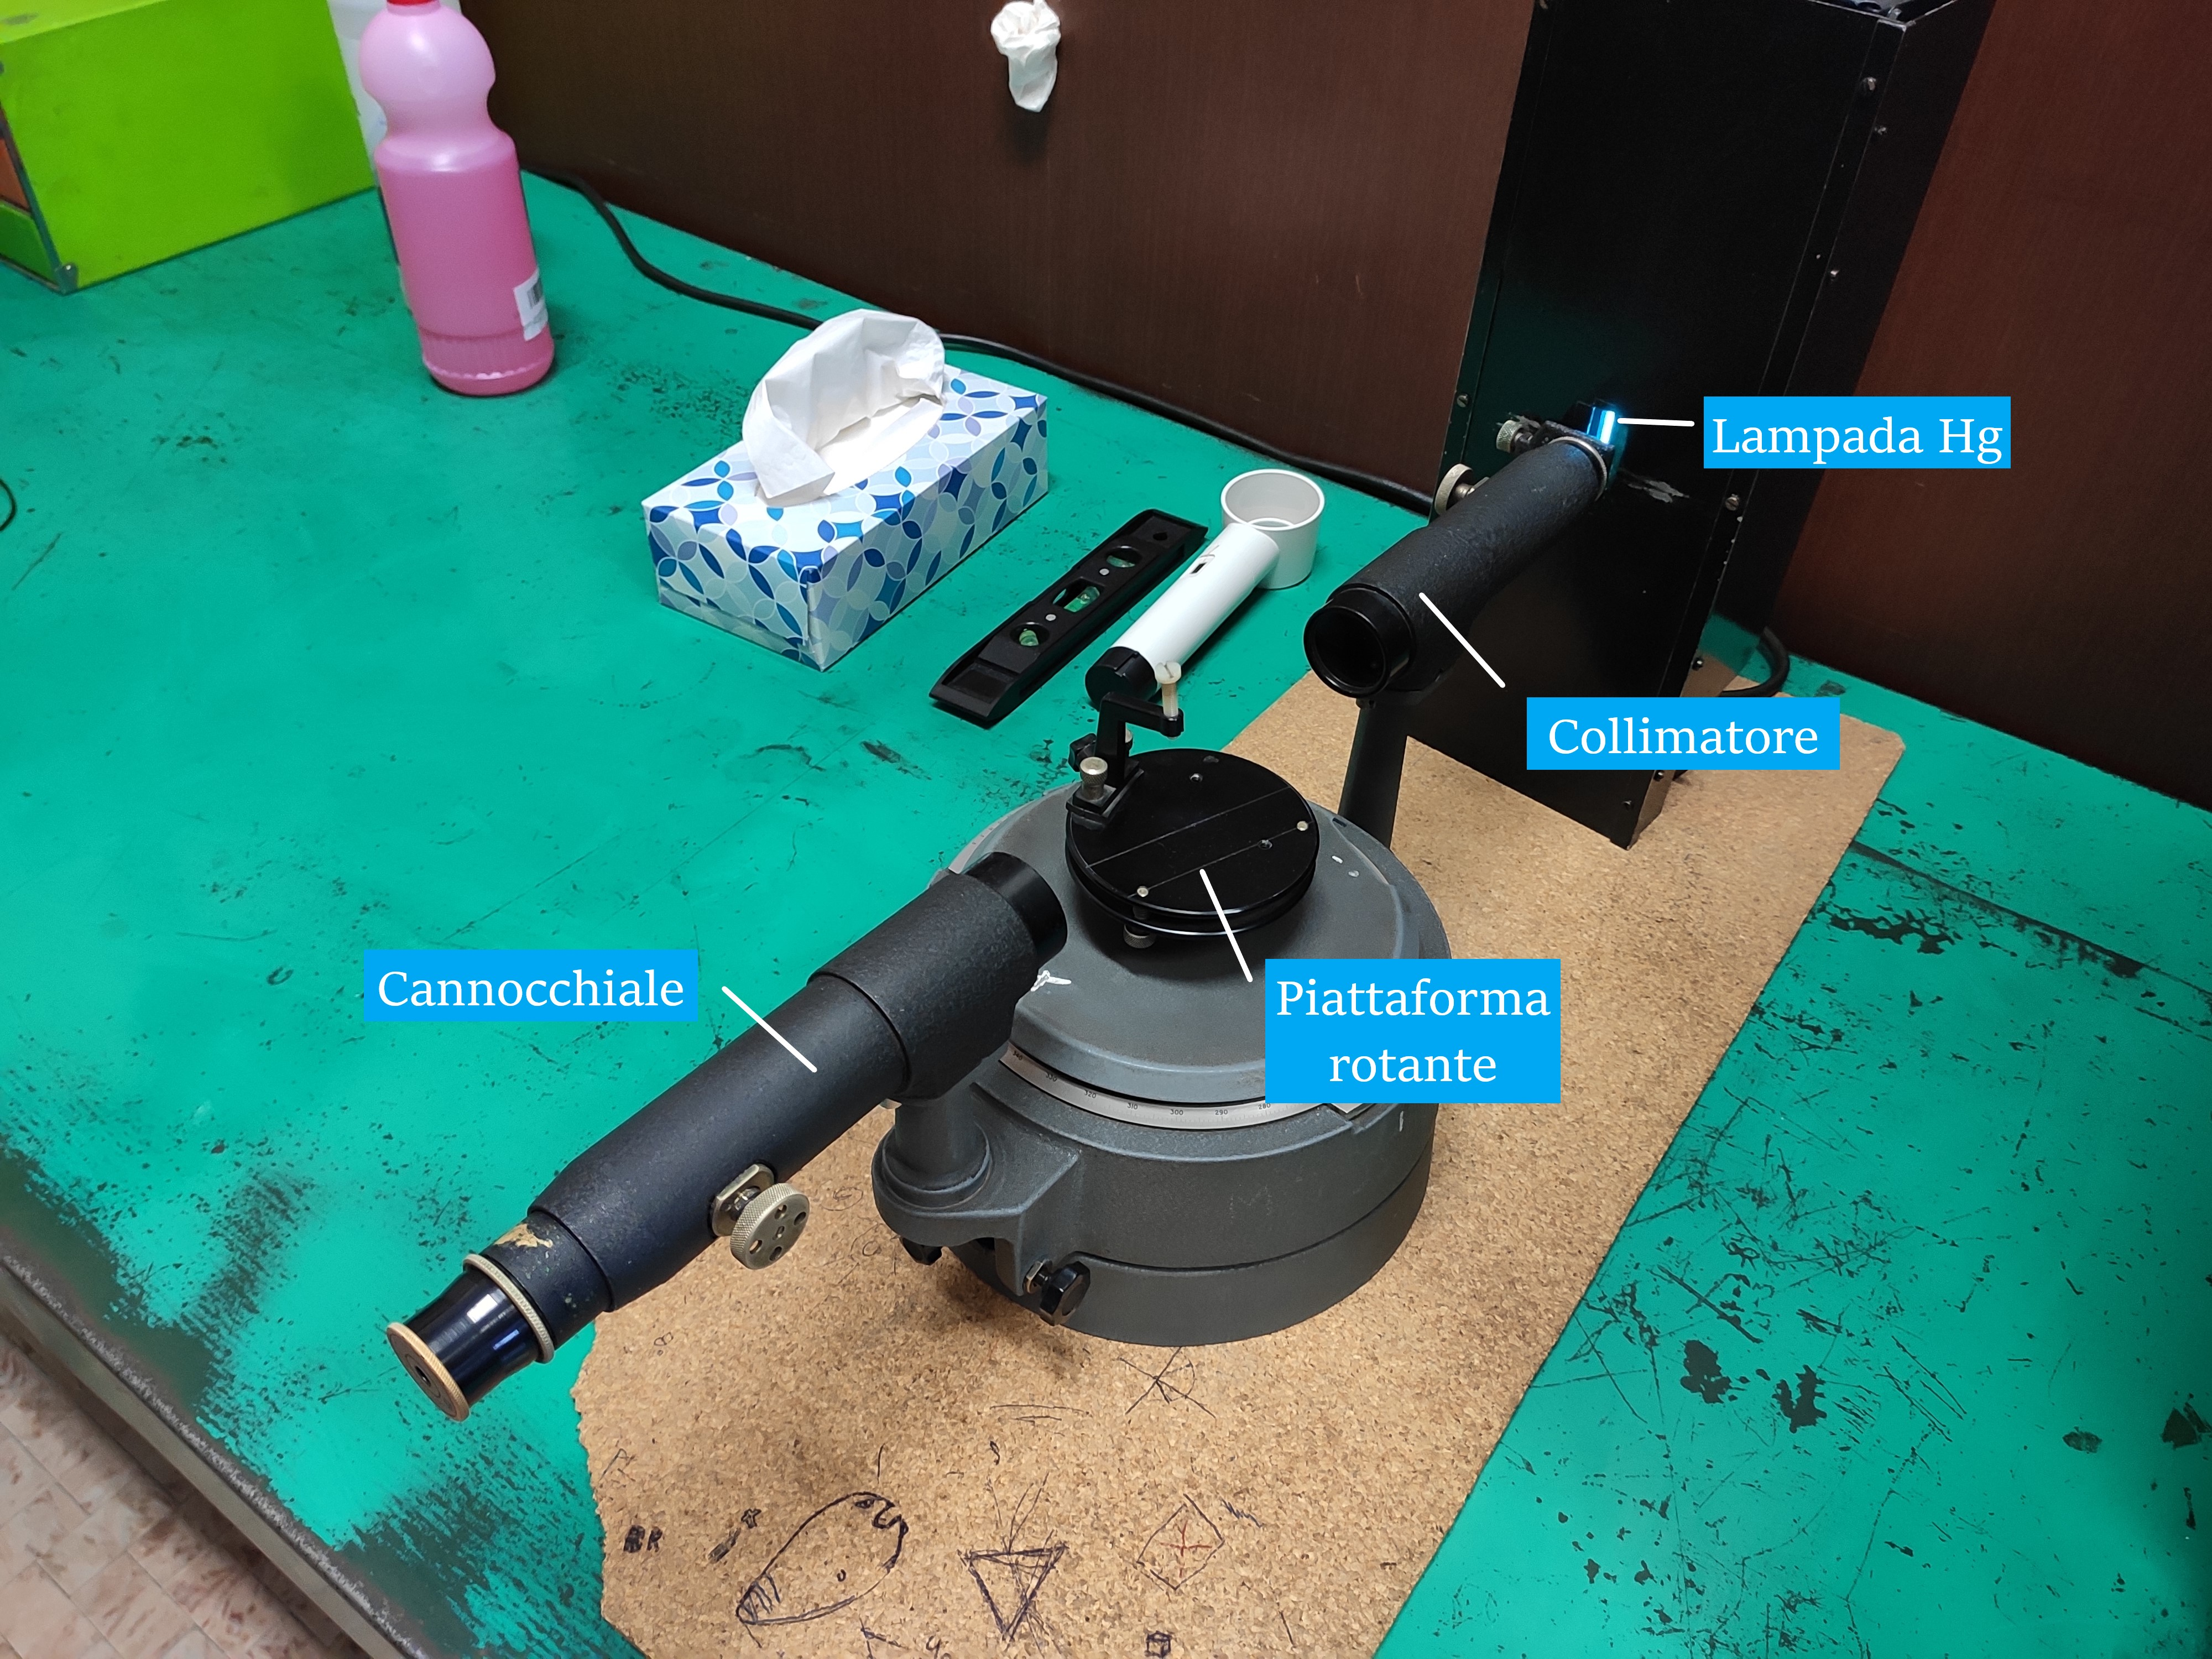
\includegraphics[width=0.6\linewidth]{FotoPrisma1}
  \caption{Foto dell'apparato sperimentale}
  \label{Foto_grande}
\end{figure}

L'apparato sperimentale (Figura \ref{Foto_grande}) è analogo a quello usato per l'esperimento del reticolo: uno spettrometro, munito di un collimatore e di una scala graduata angolare fissa, sul quale sono montati un cannocchiale mobile e una piattaforma mobile, entrambi liberi di ruotare e dotati di noni (Figura \ref{Foto_nonio}) per leggere la loro posizione angolare rispetto alla scala graduata. I noni usati in laboratorio permettono di leggere la scala graduata con una sensibilità di $30''$. Tuttavia, essendo le righe del nonio molto vicine tra loro e difficili da leggere, anche per via dell'errore dovuto alla parallasse, in questo esperimento è stato scelto di considerare solo le tacche corrispondenti ai primi d'arco. La sensibilità effettiva dei noni è quindi di $1'$.

\begin{figure}[h]
  \centering
  \includegraphics[width=0.5\linewidth]{FotoPrisma5}
  \caption{Foto del nonio}
  \label{Foto_nonio}
\end{figure}

\vspace{5mm}

La lampada è un tubo trasparente riempito di gas (in questo caso vapori di Mercurio) con degli elettrodi posti agli estremi. La differenza di potenziale tra gli elettrodi, quando sufficientemente elevata, provoca la ionizzazione degli atomi del gas. Gli elettroni eccitati tornano quindi al loro livello energetico originario, cedendo l'energia acquistata rilasciando un fotone. Le lunghezze d'onda di cui è composta la luce dipendono dagli atomi presenti nel gas.

\vspace{5mm}

Il collimatore è uno strumento che focalizza la luce proveniente dalla lampada in un fascio di luce parallela, grazie ad una fenditura regolabile, che permette di regolare la quantità di luce in ingresso, e ad una lente anch'essa regolabile per focalizzare la luce.

\vspace{5mm}

Il cannocchiale, libero di ruotare attorno alla piattaforma, permette di vedere la luce in uscita dal collimatore o dal prisma. È dotato di un crocifilo, per ''centrare'' il fascio di luce in entrata al centro del cannocchiale ruotando quest'ultimo, e grazie a due noni posti ai due lati del supporto rotante è possibile leggere la sua posizione angolare rispetto alla scala graduata. 

\vspace{5mm}

Il prisma utilizzato, a base triangolare, è realizzato in un materiale solido e trasparente. La faccia opposta all'angolo $\alpha$ è stata oscurata con un pezzo di nastro adesivo per evitare confusione ed eventuali errori.

\vspace{5mm}

All'inizio dell'esperimento è stato regolato il cannocchiale, mettendo a fuoco un edificio molto lontano visto attraverso una finestra, per focalizzare raggi di luce provenienti dall'infinito. A quel punto, posizionando il cannocchiale di fronte al collimatore in modo da vedere direttamente il fascio di luce della lampada $Hg$ (Figura 3), è stata fatta la regolazione del collimatore. Infine, utilizzando una livella a bolla, il supporto sulla piattaforma è stato regolato in modo tale da essere perfettamente orizzontale, manipolando tre apposite viti.

\vspace{5mm}

\begin{figure}[h]
  \centering
  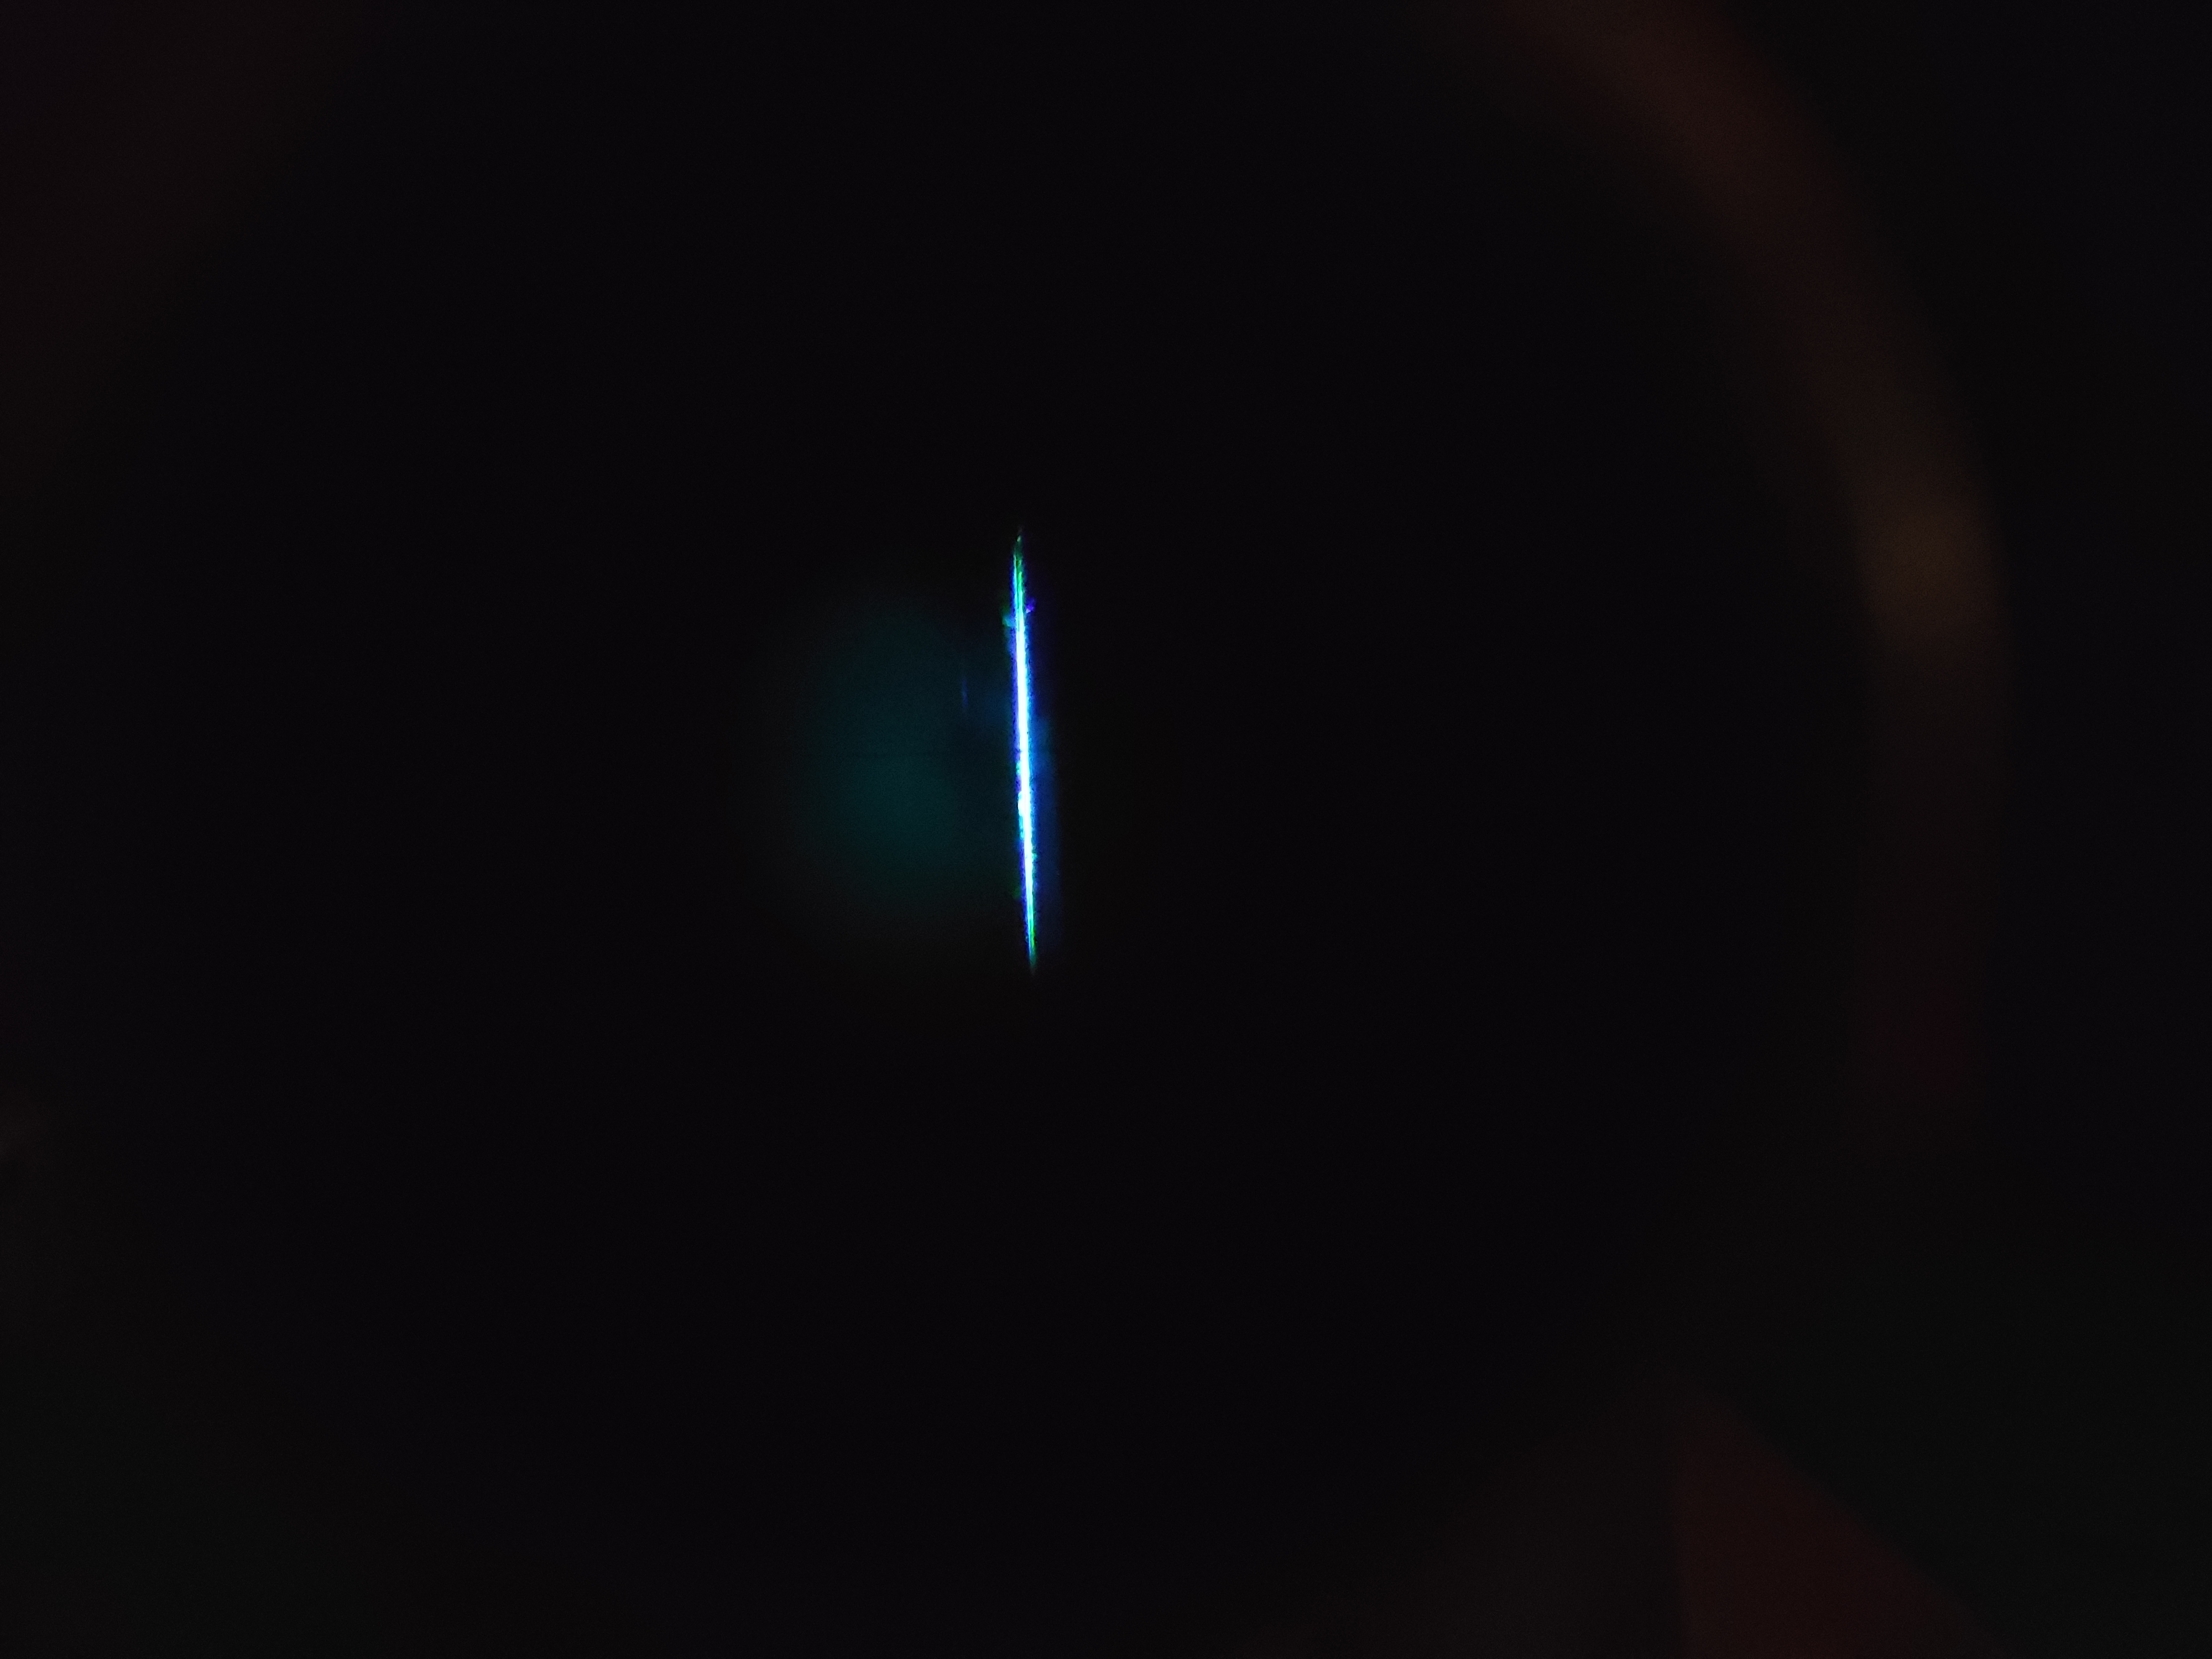
\includegraphics[width=0.5\linewidth]{FotoPrisma2}
  \caption{Il fascio di luce in uscita dal collimatore, visto dal cannocchiale}
\end{figure}

\section{Misura dell'angolo $\theta _0$}

Mantenendo il cannocchiale di fronte al collimatore, è stato centrato il fascio di luce al centro del crocifilo ed è stata misurata la posizione angolare del cannocchiale usando il relativo nonio (il cannocchiale è in realtà dotato di due diversi noni diametralmente opposti, quindi occorre avere cura di considerare sempre lo stesso. In questo esperimento è stato usato il nonio alla sinistra del cannocchiale).

Sono state fatte 10 misure di questa grandezza:

\vspace{5mm}

\begin{table}[h!]
\centering
\begin{tabular}{ | c | c | }
  \hline
   $\#$ & $\theta _0 (^{\circ})$ \\
  \hline
  1 & $58^{\circ} 45'$ \\
  2 & $58^{\circ} 44'$ \\
  3 & $58^{\circ} 46'$ \\
  4 & $58^{\circ} 46'$ \\
  5 & $58^{\circ} 45'$ \\
  6 & $58^{\circ} 44'$ \\
  7 & $58^{\circ} 45'$ \\
  8 & $58^{\circ} 45'$ \\
  9 & $58^{\circ} 45'$ \\
  10 & $58^{\circ} 45'$ \\
  \hline
  Media & $58^{\circ} 45'$ \\
  Dev. st. & $00^{\circ} 00' 38''$ \\
  $\sigma$ & $00^{\circ} 01'$ \\
  \hline
\end{tabular}
  \caption{Misura di $\theta _0$}
  \label{table:1}
\end{table}

L'incertezza ottenuta con la deviazione standard, pari a $38''$, è minore della sensibiltà del nonio. È stato quindi deciso di prendere come incertezza per l'angolo $\theta _0$ un primo.

\section{Misura dell'angolo $\alpha$}

A questo punto dell'esperimento il prisma è stato posizionato sulla piattaforma mobile e fissato a quest'ultima con un apposito fermo.

\vspace{5mm}

Per fare questa misura il cannocchiale è stato posizionato in modo da formare un angolo acuto con il collimatore (Figura \ref{angolo_acuto}). Ruotando la piattaforma mobile, il prisma è stato quindi posizionato in modo tale che il fascio di luce, riflesso sulla faccia del prisma, fosse visibile nel cannocchiale. Fissato quindi il cannocchiale e annotata la posizione della piattaforma, la piattaforma è stata fatta ruotare fino a ritrovare, nel cannocchiale, lo stesso fascio di luce riflesso sulla faccia del prisma adiacente alla prima rispetto all'angolo $\alpha$. La rotazione $\Delta \theta$ del prisma è legata all'angolo $\alpha$ dalla relazione $\alpha=180^{\circ}-\Delta \theta$, facilmente intuibile da semplici considerazioni geometriche (Figura \ref{SchemaRiflessione}).

\begin{figure}[h]
  \centering
  \includegraphics[width=0.7\linewidth]{FotoPrisma3}
  \caption{Foto dell'apparato sperimentale, con il cannocchiale posizionato ad angolo acuto con il collimatore}
  \label{angolo_acuto}
\end{figure}

\begin{figure}[h]
  \centering
  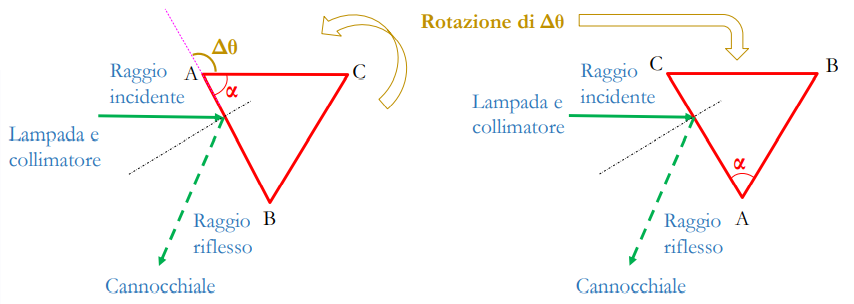
\includegraphics[width=0.7\linewidth]{Schema_Prisma_2}
  \caption{Schema della rotazione del prisma durante la misura di $\alpha$}
  \label{SchemaRiflessione}
\end{figure}

\pagebreak

Sono state fatte 5 misure:

\vspace{5mm}


\begin{table}[h!]
\centering
\begin{tabular}{ | c | c | c | c | }
  \hline
  $\theta _1 (^{\circ})$ & $\theta _2 (^{\circ})$ & $\Delta \theta (^{\circ})$ & $\alpha (^{\circ})$ \\
  \hline
  $355^{\circ} 50'$ & $235^{\circ} 49'$ & $120^{\circ} 01'$ & $59^{\circ} 59'$ \\
  $355^{\circ} 50'$ & $235^{\circ} 50'$ & $120^{\circ} 00'$ & $60^{\circ} 00'$ \\
  $355^{\circ} 52'$ & $235^{\circ} 52'$ & $120^{\circ} 00'$ & $60^{\circ} 00'$ \\
  $11^{\circ} 44'$ & $251^{\circ} 44'$ & $120^{\circ} 01'$ & $60^{\circ} 00'$ \\
  $11^{\circ} 43'$ & $251^{\circ} 44'$ & $119^{\circ} 59'$ & $60^{\circ} 01'$ \\
  \hline
  && Media & $60^{\circ} 00'$ \\
  && Dev. st. & $00^{\circ} 00' 38''$ \\
  && $\sigma$ & $00^{\circ} 01'$ \\
  \hline
\end{tabular}
  \caption{Misura di $\alpha$}
  \label{table:1}
\end{table}

Durante la quarta misura, il banco da lavoro è stato urtato accidentalmente, cosa che ha causato un lieve movimento del prisma rispetto alla piattaforma rotante. La misura è stata quindi ripetuta. Non ci sono state ulteriori conseguenze.

Similarmente a quanto fatto per la misura di $\theta _0$, si è deciso di prendere come incertezza dell'angolo $\alpha$ un primo.


\section{Misura dell'angolo di deviazione minima}

Per la ricerca dell'angolo di deviazione minima è necessario posizionare il prisma in modo tale che la luce rifratta non esca dal prisma dalla faccia oscurata. Posizionato il prisma in tale maniera, si procede alla ricerca delle righe della lampada $Hg$ ad occhio nudo e, una volta trovate, si ruota il cannocchiale in posizione tale da poterle vedere (Figura \ref{Refraction}).

In questo esperimento erano visibili 7 righe:

\begin{itemize}
  \item Viola
  \item Blu
  \item Verde acqua
  \item Verde
  \item Doppietto del giallo
  \item Rosso
\end{itemize}

Scelta una riga, è stato trovato l'angolo di deviazione minima ruotando la piattaforma mobile fino a trovare il punto di inversione del moto e ed è stato centrato il cannocchiale su quella riga. Per ogni riga sono state fatte 5 misure. A quel punto è stata fatta una media delle misure, e la loro deviazione standard è stata usata come incertezza della media (come nelle misure precedenti, nel caso in cui questa fosse più piccola della sensibilità del nonio, quest'ultima è stata usata come incertezza). È stato quindi calcolato l'angolo $\delta$, ricordando che $\delta = \theta - \theta _0$, con relativa incertezza $\sigma \delta = \sqrt{\sigma \theta ^2 + \sigma \theta_0 ^2}$.

A questo punto abbiamo potuto calcolare l'indice di rifrazione $n (\lambda)$ usando la formula precedentemente ricavata

\[n(\lambda) = \frac{\textrm{sen}\, \frac{\delta + \alpha}{2}}{\textrm{sen}\, \frac{\alpha}{2}}\]

 e la relativa incertezza con la formula della propagazione degli errori

\[\sigma n = \sqrt{\left( \frac{\partial n}{\partial \alpha}\sigma \alpha \right)^2 + \left( \frac{\partial n}{\partial \delta}\sigma \delta \right)^2} = \sqrt{\left( \frac{\frac{1}{2}\textrm{cos}\, \frac{\delta + \alpha}{2}\textrm{sen}\, \frac{\alpha}{2} - \frac{1}{2}\textrm{sen}\, \frac{\delta + \alpha}{2}\textrm{cos}\, \frac{\alpha}{2}}{\textrm{sen}^2\, \frac{\alpha}{2}} \sigma \alpha  \right)^2 + \left( \frac{\frac{1}{2}\textrm{cos}\, \frac{\delta + \alpha}{2}}{\textrm{sen}\, \frac{\alpha}{2}} \sigma \delta \right)^2}\]

\begin{table}[h!]
\centering
\begin{tabular}{ | c | c | c | c | c | c | c | c | }
  \hline
   $\#$ & Viola & Blu & Verde acqua & Verde & Giallo1 & Giallo2 & Rosso \\
  \hline
  1 & $132^{\circ} 54'$ & $130^{\circ} 30'$ & $127^{\circ} 43'$ & $126^{\circ} 02'$ & $125^{\circ} 20'$ &  $125^{\circ} 19'$ &  $123^{\circ} 31'$ \\
  2 & $132^{\circ} 54'$ & $130^{\circ} 30'$ & $127^{\circ} 42'$ & $126^{\circ} 02'$ & $125^{\circ} 20'$ &  $125^{\circ} 16'$ &  $123^{\circ} 30'$ \\
  3 & $132^{\circ} 54'$ & $130^{\circ} 30'$ & $127^{\circ} 42'$ & $126^{\circ} 03'$ & $125^{\circ} 19'$ &  $125^{\circ} 15'$ &  $123^{\circ} 31'$ \\
  4 & $132^{\circ} 53'$ & $130^{\circ} 30'$ & $127^{\circ} 44'$ & $126^{\circ} 03'$ & $125^{\circ} 19'$ &  $125^{\circ} 14'$ &  $123^{\circ} 31'$ \\
  5 & $132^{\circ} 54'$ & $130^{\circ} 29'$ & $127^{\circ} 43'$ & $126^{\circ} 02'$ & $125^{\circ} 20'$ &  $125^{\circ} 17'$ &  $123^{\circ} 32'$ \\
  \hline
  Media & $132^{\circ} 53' 48''$ & $130^{\circ} 29' 48''$ & $127^{\circ} 42' 48''$ & $126^{\circ} 02' 24''$ & $125^{\circ} 19' 36''$ &  $125^{\circ} 16' 12''$ &  $123^{\circ} 31'$ \\
  Dev. st. & $00^{\circ} 00' 24''$ & $00^{\circ} 00' 24''$ & $00^{\circ} 00' 45''$ & $00^{\circ} 00' 29''$ & $00^{\circ} 00' 29''$ & $00^{\circ} 01' 43''$ & $00^{\circ} 00' 38''$ \\
  $\sigma$ &  $00^{\circ} 01'$ & $00^{\circ} 01'$ & $00^{\circ} 01'$ & $00^{\circ} 01'$ & $00^{\circ} 01'$ & $00^{\circ} 01' 43''$ & $00^{\circ} 01'$ \\
  \hline
  $\delta (^{\circ} dec.)$ & $74,13$ & $71,73$ & $68,95$ & $67,28$ & $66,57$ & $66,52$ & $64,77$ \\
  $\sigma \delta $ & $0,024$ & $0,024$ & $0,024$ & $0,024$ & $0,024$ & $0,033$ & $0,024$ \\
  \hline
  $n (\lambda)$ & $1,84192$ & $1,8252$ & $1,80479$ & $1,7921$ & $1,7865$ & $1,7861$ & $1,7721$ \\
  $\sigma n$ & $0,00013$ & $0,0003$ & $0,00002$ & $0,0002$ & $0,0002$ & $0,0003$ & $0,0002$ \\
  \hline
\end{tabular}
  \caption{Misure dell'angolo $\theta$ per le 7 righe visibili}
  \label{table:1}
\end{table}

\begin{figure}[h!]
  \centering
  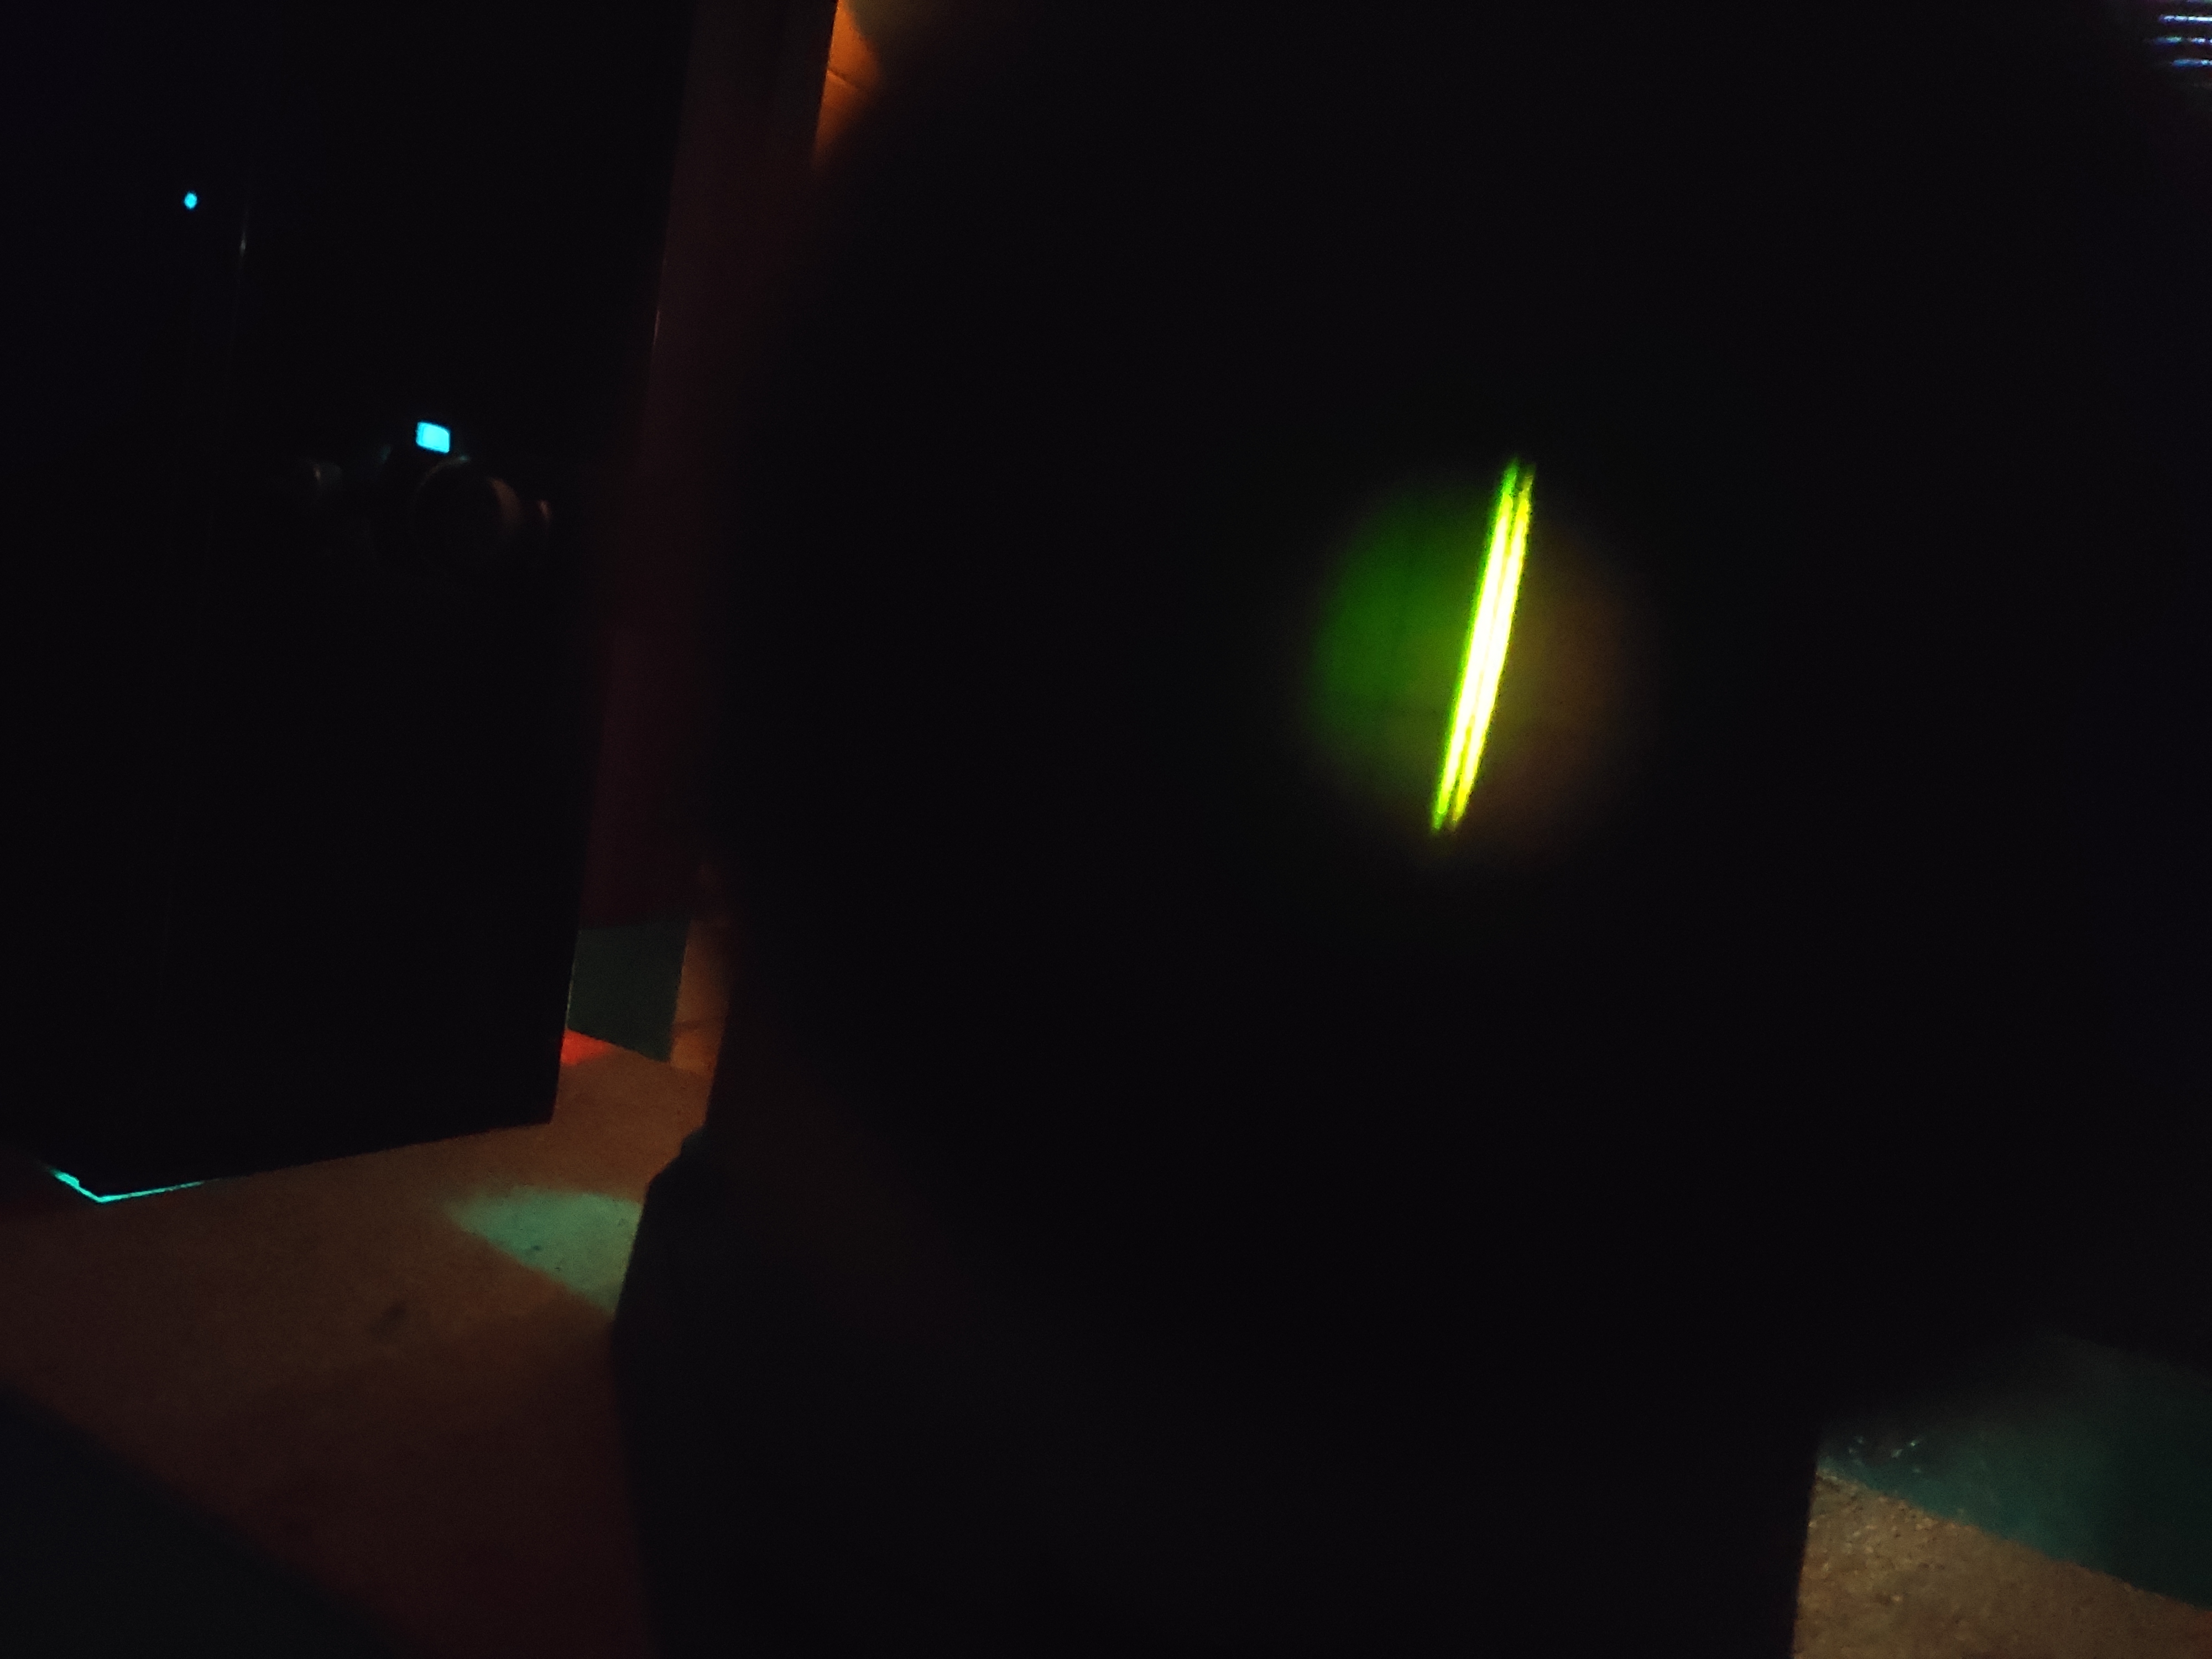
\includegraphics[width=0.7\linewidth]{FotoPrisma4}
  \caption{Foto del fascio di luce rifratto dal prisma. Visibile il doppietto del giallo}
  \label{Refraction}
\end{figure}

\clearpage

\section{Analisi dei dati}

Trovati i valori di $n (\lambda)$, resta da verificare che seguano la relazione di Cauchy

\[n(\lambda)=a+\frac{b}{\lambda ^2}\]

I valori di $\lambda$ per la lampada $Hg$ con relativa incertezza sono stati trovati nell'esperimento del reticolo, e sono 

\begin{table}[h!]
\centering
\begin{tabular}{ | c | c | c | }
  \hline
  Colore & $\lambda (m)$ & $\sigma \lambda (m)$ \\
  \hline
  Viola & $4,08 \cdot 10^{-6}$ & $1,1 \cdot 10^{-7}$ \\
  Blu & $4,36 \cdot 10^{-6}$ & $1,1 \cdot 10^{-7}$ \\
  Verde & $5,47 \cdot 10^{-6}$ & $8 \cdot 10^{-8}$ \\
  Giallo1 & $5,75 \cdot 10^{-6}$ & $8 \cdot 10^{-8}$ \\
  Giallo2 & $5,80 \cdot 10^{-6}$ & $8 \cdot 10^{-8}$ \\
  \hline
\end{tabular}
  \caption{Le lunghezze d'onda trovate nell'esperimento del reticolo}
  \label{table:1}
\end{table}

Durante l'esperimento del reticolo non sono state misurate le lunghezze d'onda per le righe del verde acqua e del rosso. Al loro posto sono stati usati i valori tabulati (rispettivamente $4,96010 \cdot 10^{-6} m$ e $6,90746 \cdot 10^{-6} m$) riportati dal NIST (National Institute of Standards and Technology), trascurandone l'incertezza. In entrambi i casi sono state scelte le righe più alta intensità relativa. 

Abbiamo usato il metodo dei minimi quadrati, con 

\[x=\frac{1}{\lambda ^2} \quad \textrm{e} \quad y=n\]

\[\sigma y = \sigma n + b_{test} \cdot \sigma \frac{1}{\lambda ^2} \quad \textrm{dove} \quad \sigma \frac{1}{\lambda ^2}=2 \cdot \frac{\sigma \lambda}{\lambda ^3} \quad \textrm{e} \quad  b_{test} = \frac{n_{rosso}-n_{viola}}{\frac{1}{\lambda _{r}^2}-\frac{1}{\lambda _{v}^2}}\]

\begin{table}[h!]
\centering
\begin{tabular}{ | c | c | c | c | c | c | c | c | }
  \hline
  Colore & $\lambda (m)$ & $\sigma \lambda (m)$ &  $\frac{1}{\lambda^2} (\frac{1}{m^2})$ & $\sigma \frac{1}{\lambda^2} (\frac{1}{m^2})$ & $n(\lambda)$ & $\sigma n$ & $\sigma y$\\
  \hline
  Viola & $4,08 \cdot 10^{-6}$ & $1,1 \cdot 10^{-7}$ & $6,0 \cdot 10^{10}$ & $3 \cdot 10^9$ & $1,84192$ & $0,00013$ & $0,00591$\\
  Blu & $4,36 \cdot 10^{-6}$ & $1,1 \cdot 10^{-7}$ & $5,3 \cdot 10^{10}$ & $3 \cdot 10^9$ & $1,8252$ & $0,0003$ & $0,00499$\\
  Verde acqua & $4,96010 \cdot 10^{-6}$ && $4,06 \cdot 10^{10}$ && $1,80479$ & $0,00002$ & $0,00002$\\
  Verde & $5,47 \cdot 10^{-6}$ & $8 \cdot 10^{-8}$ & $3,34 \cdot 10^{10}$ & $9 \cdot 10^8$ & $1,79207$ & $0,00019$ & $0,00182$\\
  Giallo1 & $5,75 \cdot 10^{-6}$ & $8 \cdot 10^{-8}$ & $3,02 \cdot 10^{10}$ & $9 \cdot 10^8$ & $1,7865$ & $0,0002$ & $0,00164$\\
  Giallo2 & $5,80 \cdot 10^{-6}$ & $8 \cdot 10^{-8}$ & $2,97 \cdot 10^{10}$ & $8 \cdot 10^8$ & $1,7861$ & $0,0003$ & $0,00167$\\
  Rosso & $6,908 \cdot 10^{-6}$ && $2,10 \cdot 10^{10}$ && $1,7721$ & $0,0002$ & $0,0002$\\
  \hline
\end{tabular}
  \caption{I dati per la regressione lineare}
  \label{table:1}
\end{table}

\[b_{test}=1,78 \cdot 10^{-12}\]

\begin{figure}[h!]
  \centering
  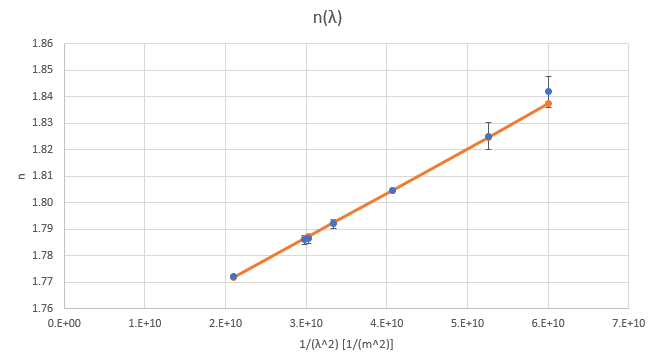
\includegraphics[width=0.9\linewidth]{GraficoPrisma2}
  \caption{Grafico della regressione lineare. In blu i punti misurati, in arancio la linea creata dal modello}
\end{figure}

I risultati della regressione lineare sono:

\[a=1,74 \pm 0,03\]
\[b=1,6 \cdot 10^{-12} \pm 7 \cdot 10^{-13} m^2\]

Le tabelle relative alla regressione e al test del $\chi ^2$ sono in appendice.

\begin{center}
\begin{tabular}{ | c | c |  }
  \hline
  $\chi ^2$ & $4,05$\\
  g.d.l. & $5$\\
  $\chi ^2$ ridotto & $0,81$\\
  \hline
  P (0,8) & $55 \%$\\
  \hline
\end{tabular}
\end{center}

\section{Conclusioni}
L'analisi dei dati mostra che i valori di $n(\lambda)$ misurati seguono la relazione di Cauchy. Infatti otteniamo un $\chi^2$ con una probabilità del 55\% che consideriamo accettabile alla soglia al 5\%. Ci riteniamo quindi sicuri della bontà delle misure effettuate e possiamo concludere che l'esperimento si è concluso con successo.

\clearpage

\section{Appendice}

\begin{figure}[h!]
  \centering
  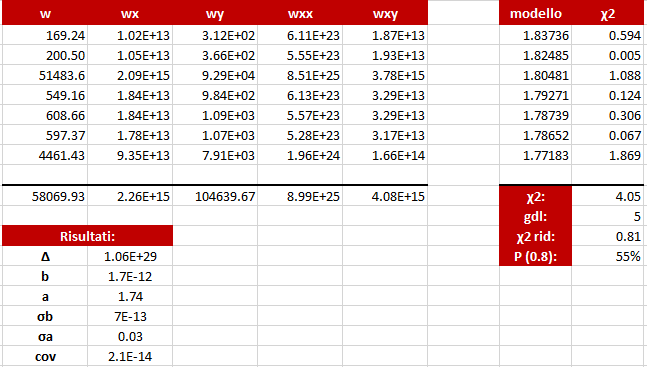
\includegraphics[width=\linewidth]{Prisma_app}
  \caption{Tabella della regressione lineare, con risultati e test del $\chi ^2$}
\end{figure}

\end{document}
